\chapter{Results}
\label{chapter:results}

This chapter describes the experiments in terms of reproducible steps, settings, parameters, and conditions, as well as present and discuss their results.

Ultimately the experiments aim to study transfer learning in the specific domain of skin lesion classification, as well as compare its efficacy against simpler and more traditional learning schemes, by training and testing several models of different architectures and drawing helpful conclusions about the use of transfer learning techniques.

\section{VGG16 Transfer Learning Experiments}

Based on the transfer learning techniques introduced in chapter \ref{chapter:sota}, models of the VGG16 architecture pre-trained on ImageNet will be explored in order to repurpose the weights to a new model for skin lesion classification and draw conclusions about its efficacy.

It is hypothesized that extracting features from lower layers of models trained for ImageNet classification can provide good performance, because the former presumably provide low-level features (e.g. shapes or lines) that are still useful for skin lesion classification whereas the latter provide very high-level concepts (e.g. dogs, cats) that are most relevant for classification in the ImageNet domain and otherwise needs fine-tuning to the target dataset.

The basic unit in traditional \ac{CNN} architectures like VGG16 is the convolutional block, which is typically comprised by a stack of convolutional layers and one pooling layer for downsampling. These convolutional blocks are then further stacked together to progressively output higher level feature maps at the end of each block.

To verify this, one can run a sample input (figure \ref{fig:sample_input}) through the original VGG16 model pre-trained on ImageNet and visualize the activations at the end of each block (after its pooling layer).

\begin{figure}[ht]
    \centering
    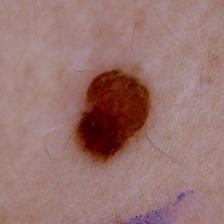
\includegraphics[width=0.3\textwidth]{figs/sample_input.jpg}
    \caption{A sample of the ISIC2018 train set showing a clear separation of background (skin) and foreground (lesion).}
    \label{fig:sample_input}
\end{figure}

As expected, the features detected in the early layers of the network (figure \ref{fig:vgg16_block1}) activate for low level concepts like shapes (the border around the lesion), background (the skin), and foreground (the lesion itself).

\begin{figure}[ht]
    \centering
    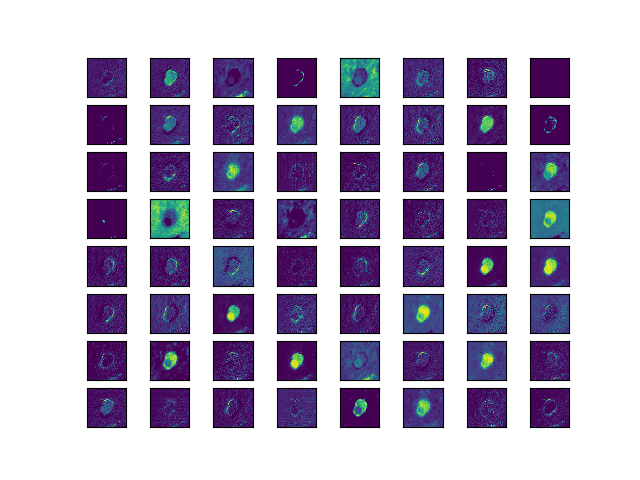
\includegraphics[width=0.7\textwidth]{figs/vgg16_block1.png}
    \caption{The 64 feature maps at the end of block 1 of the VGG16 model exactly as trained on ImageNet.}
    \label{fig:vgg16_block1}
\end{figure}

On the other hand at the last block of the network the feature maps exhibit much higher level (and low dimensional) concepts (figure \ref{fig:vgg16_block5}) incomprehensible to the human eye.

\begin{figure}[ht]
    \centering
    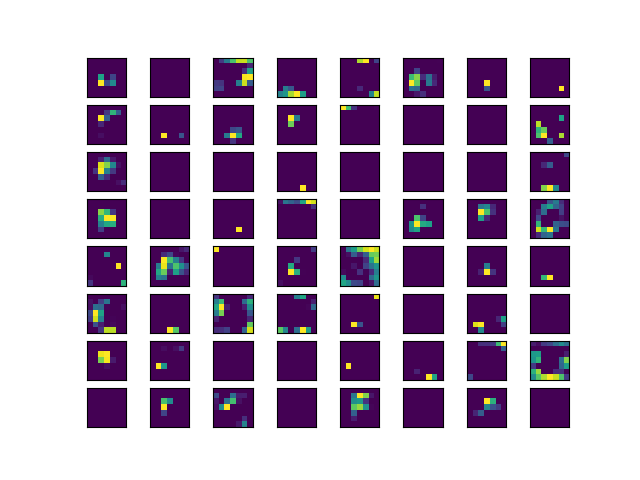
\includegraphics[width=0.7\textwidth]{figs/vgg16_block5.png}
    \caption{64 of the feature maps at the end of block 5 of the VGG16 model exactly as trained on ImageNet.}
    \label{fig:vgg16_block5}
\end{figure}

Clearly, successful transfer learning from the VGG16 pre-trained model is highly dependent on the layer up to which weights are extracted from. Presumably extracting all layers and fine-tuning them to the target dataset will always work, but in some cases it might be useful to extract only a subset of the features in order to produce a smaller model for applications where space (occupied by the model) and computation (required by the forward pass of an inherently deeper model) are at a premium (e.g. smartphones). Both of these cases (and more) will be explored.

To do this it is helpful to define two variables:

\begin{itemize}
    \item the number of the layer $e$ up to which parameters will be extracted (or used) from will be sampled from $e \in \{18,14,10,6,3\}$;
    \item the number of the layer $f$ up to which parameters will be frozen will be sampled from $f \in \{18,14,10,6,3,0\}$;
\end{itemize}

VGG16 is named after its 16 layers of parameters found in convolutional layers (13) and fully-connected layers (3). However, for narrative purposes and easier reproducibility, the variables $e$ and $f$ will refer to the index of the layers as implemented in \verb|tf.keras.applications.vgg16|\footnote{\url{https://www.tensorflow.org/api_docs/python/tf/keras/applications/VGG16}}. Of course, input layers and pooling layers are inherently not parameterized. Specifically, the \verb|tf.keras.applications.vgg16| implementation of the VGG16 model pre-trained on ImageNet organizes layers as such:

\begin{itemize}
    \item Layer 0 is the input layer (\verb|input_1|) and will not be considered for extraction as it merely represents the original input;
    \item Layers 1-3 are the first convolutional block (\verb|block1_conv1|, \verb|block1_conv2|, \verb|block1_pool|);
    \item Layers 4-6 are the second convolutional block (\verb|block2_conv1|, \verb|block2_conv2|, \verb|block2_pool|);
    \item Layers 7-10 are the third convolutional block (\verb|block3_conv1|, \verb|block3_conv2|, \verb|block3_conv3|, \verb|block3_pool|);
    \item Layers 11-14 are the fourth convolutional block (\verb|block4_conv1|, \verb|block4_conv2|, \verb|block4_conv3|, \verb|block4_pool|);
    \item Layers 15-18 are the fifth convolutional block (\verb|block5_conv1|, \verb|block5_conv2|, \verb|block5_conv3|, \verb|block5_pool|);
    \item Layers 19-22 are non-convolutional layers (\verb|flatten|, \verb|fc1|, \verb|fc2|, \verb|predictions|) and will not be considered for extraction.
\end{itemize}

\subsection{Total Feature Extraction without Fine Tuning}

Arguably the simplest case is to extract and freeze all layers (i.e. $e = f = 18$), feed them to the classifier, and effectively only train the classifier. Specifically, training follows the methodology:

% TODO: fix extract/freeze part
\begin{enumerate}
    \item Standardize training and validation samples relative to ImageNet;
    \item Some parameters are transfered from pre-trained models and otherwise initialized according to Xavier initialization;
    \item Define network architecture:
        \begin{enumerate}
            \item Extract and freeze layers from the pre-trained model according to the specific experiment at hand;
            \item Use global average pooling to reduce the number of parameters before the classifier based on fully-connected layers;
            \item Use one fully-connected layer of 512 ReLU-activated neurons;
            \item Use one fully-connected layer of 1 sigmoid-activated neuron for binary classification.
        \end{enumerate}
    \item Mini-batch \ac{SGD} with momentum $\gamma = 0.9$:
        \begin{itemize}
            \item Binary cross entropy cost function and explicit L2 regularization with $\lambda \in [0.0001, 0.005]$ spaced evenly on a log scale;
            \item 32 samples batches;
            \item Initial learning rate $\eta = 10^{-4}$ that decays by a factor of $10$ if the validation accuracy has not improved $+10^{-3}$ in the last $10$ epochs;
            \item Shuffle the $m$ samples every epoch;
            \item Train for a maximum of 1000 epochs, stopping early if the loss has not changed $\pm 10^{-3}$ in the last $30$ epochs.
        \end{itemize}
    \item Grid-search model selection based on the accuracy as measured on a fixed validation set;
    \item Final models will be evaluated and compared primarily using accuracy as measured on the test set.
\end{enumerate}

Surprisingly models converge nicely and quickly (e.g. figure \ref{fig:vgg16_total_convergence}) and already give very good results overall (table \ref{table:vgg16_total}).

\begin{figure}[ht]
    \centering
    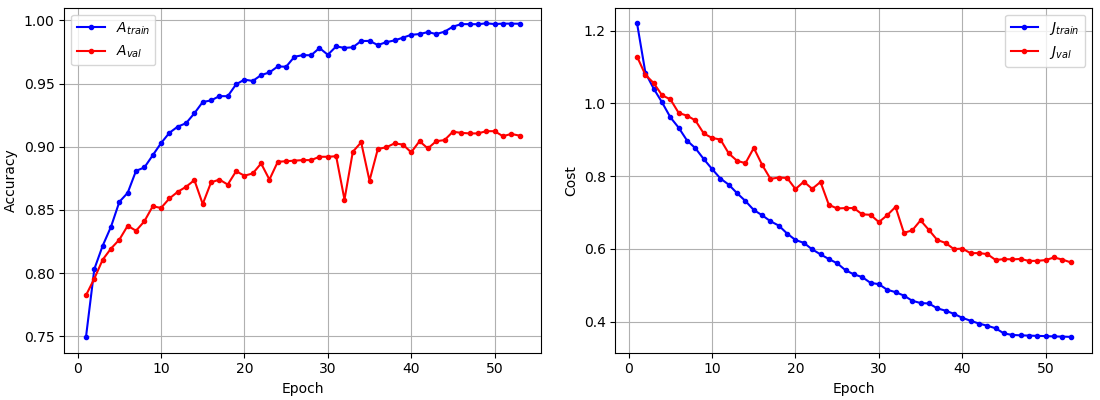
\includegraphics[width=0.9\textwidth]{figs/vgg16_total_convergence.png}
    \caption{Convergence of a model where $e = f = 18$ and $\lambda = 0.00135721$.}
    \label{fig:vgg16_total_convergence}
\end{figure}

\begin{table}[ht]
\centering
\begin{tabular}{ |c|c|c|c|c|c|c|c|c|c| }
\hline
$e$ & $f$ & $\lambda$ & $A_{train}$ & $A_{val}$ & $A_{test}$ & AUC & Precision & Recall & F1-Score \\
\hline
18.0 & 18.0 & 0.0001 & 1.0 & 0.914 & 0.914 & 0.914 & 0.916 & 0.914 & 0.914 \\
18.0 & 18.0 & 0.000154 & 0.995 & 0.9 & 0.911 & 0.911 & 0.914 & 0.911 & 0.911 \\
18.0 & 18.0 & 0.000239 & 1.0 & 0.911 & 0.914 & 0.914 & 0.916 & 0.914 & 0.914 \\
18.0 & 18.0 & 0.000368 & 1.0 & 0.908 & 0.915 & 0.915 & 0.917 & 0.915 & 0.915 \\
18.0 & 18.0 & 0.000569 & 0.994 & 0.904 & 0.912 & 0.912 & 0.914 & 0.912 & 0.912 \\
18.0 & 18.0 & 0.000879 & 0.998 & 0.911 & 0.915 & 0.915 & 0.918 & 0.915 & 0.915 \\
18.0 & 18.0 & 0.00136 & 0.998 & 0.911 & 0.918 & 0.918 & 0.92 & 0.918 & 0.918 \\
18.0 & 18.0 & 0.0021 & 0.994 & 0.908 & 0.915 & 0.915 & 0.917 & 0.915 & 0.915 \\
18.0 & 18.0 & 0.00324 & 0.991 & 0.902 & 0.911 & 0.911 & 0.914 & 0.911 & 0.911 \\
18.0 & 18.0 & 0.005 & 0.975 & 0.893 & 0.906 & 0.906 & 0.909 & 0.906 & 0.905 \\
\hline
 & & & $0.995\pm0.00713$ & $0.906\pm0.0061$ & $0.913\pm0.00311$ & $0.913\pm0.00311$ & $0.916\pm0.00284$ & $0.913\pm0.00311$ & $0.913\pm0.00335$ \\
\hline
\end{tabular}
\caption{Performance metrics of models when $e = 18$ and $f = 18$.}
\label{table:vgg16_total}
\end{table}

The validation curve of the L2-regularization strength $\lambda$ hyperparameter in figure \ref{fig:vgg16_total_lambda} shows these models are neither overfitting nor underfitting as $A_{val}$ is approximating $A_{train}$ well.

\begin{figure}[ht]
    \centering
    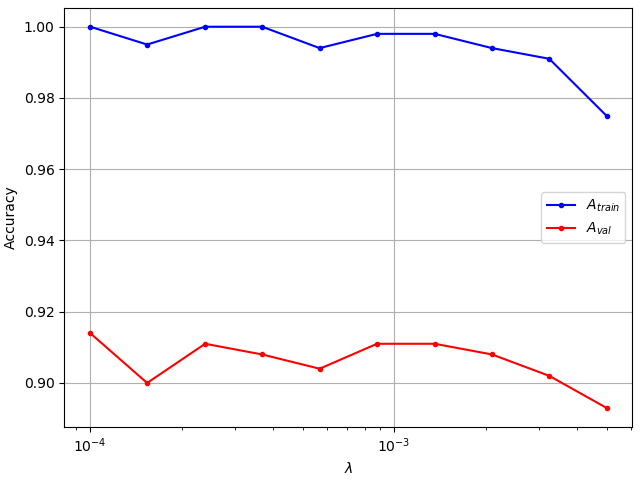
\includegraphics[width=0.6\textwidth]{figs/vgg16_total_lambda.png}
    \caption{Plot of L2-regularization strength $\lambda$ against accuracy on the test set $A_{test}$ when $e = 18$ and $f = 18$.}
    \label{fig:vgg16_total_lambda}
\end{figure}

Presumably these surprisingly good results stem from an appropriate number $m$ of training samples (relative to the number of free parameters in the network) and proper data augmentation. It is also important to remember that binary classification is a much easier optimization problem when compared to ImageNet's 1000-class classification.

Indeed, by fixating $\lambda = 0.000879$ (for example) and varying the number of samples as fractions ${0.1, 0.2, 0.3, 0.4, 0.5, 0.6, 0.7, 0.8, 0.9}$ of the total $m$ training samples it can be seen (in table \ref{table:vgg16_total_debug}) that performance increases as the number of samples increases.

% TODO: convert this to plot

\begin{table}[ht]
\centering
\begin{tabular}{ |c|c|c|c|c|c|c| }
\hline
Fraction & $A_{train}$ & $A_{val}$ & $A_{test}$ & Precision & Recall & F1-Score \\
\hline
0.1 & 0.977 & 0.771 & 0.784 & 0.784 & 0.784 & 0.784 \\
0.2 & 0.991 & 0.803 & 0.82  & 0.821 & 0.82  & 0.82  \\
0.3 & 0.973 & 0.819 & 0.835 & 0.836 & 0.835 & 0.835 \\
0.4 & 0.984 & 0.843 & 0.854 & 0.857 & 0.854 & 0.854 \\
0.5 & 0.997 & 0.863 & 0.872 & 0.872 & 0.872 & 0.872 \\
0.6 & 0.987 & 0.868 & 0.879 & 0.881 & 0.879 & 0.879 \\
0.7 & 0.996 & 0.881 & 0.889 & 0.891 & 0.889 & 0.889 \\
0.8 & 0.998 & 0.899 & 0.906 & 0.908 & 0.906 & 0.906 \\
0.9 & 0.989 & 0.894 & 0.904 & 0.906 & 0.904 & 0.904 \\
\hline
 & $0.988\pm0.00829$ & $0.849\pm0.0412$ & $0.86\pm0.0386$ & $0.862\pm0.0392$ & $0.86\pm0.0386$ & $0.86\pm0.0386$ \\
\hline
\end{tabular}
\caption{Performance metrics of models when $e = 18$, $f = 18$, $\lambda = 0.000879$ and the fraction of the number of samples $m$ is varied.}
\label{table:vgg16_total_debug}
\end{table}

\subsection{Partial Feature Extraction without Fine Tuning}

Extracting a smaller number of layers seemed promising since that would yield a smaller and faster model. Besides, presumably, the most relevant features were in the middle layers anyway. However none of the models seemed to be converging usefully, likely stuck in a local minimum with high loss (e.g. figure \ref{fig:vgg16_partial_divergence}).

\begin{figure}[ht]
    \centering
    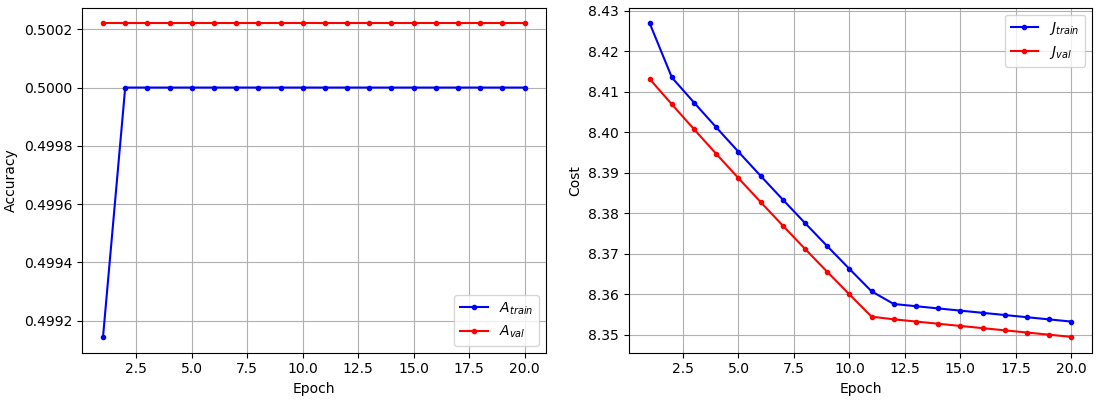
\includegraphics[width=0.8\textwidth]{figs/vgg16_partial_divergence.png}
    \caption{Partial feature extraction network (with $e = 14$, $f = 14$, $\lambda = 0.00015445$, $\eta = 10^{-4}$) not converging, stuck in a local minimum.}
    \label{fig:vgg16_partial_divergence}
\end{figure}

Accordingly, performance results (in table \ref{table:vgg16_partial}) were disappointing for any number $e < 18$ of frozen layers.

% TODO: fix table

\begin{table}[ht]
\centering
\begin{tabular}{ |c|c|c|c|c|c|c|c|c|c| }
\hline
$e$ & $f$ & $\lambda$ & $A_{train}$ & $A_{val}$ & $A_{test}$ & AUC & Precision & Recall & F1-Score \\
\hline
14.0 & 0.0 & 0.0001 & 0.5 & 0.5 & 0.5 & 0.5 & 0.25 & 0.5 & 0.334 \\
14.0 & 0.0 & 0.000154 & 0.5 & 0.5 & 0.5 & 0.5 & 0.25 & 0.5 & 0.334 \\
14.0 & 0.0 & 0.000239 & 0.5 & 0.5 & 0.5 & 0.5 & 0.25 & 0.5 & 0.334 \\
14.0 & 0.0 & 0.000368 & 0.5 & 0.5 & 0.5 & 0.5 & 0.25 & 0.5 & 0.334 \\
14.0 & 0.0 & 0.000569 & 0.5 & 0.5 & 0.5 & 0.5 & 0.25 & 0.5 & 0.334 \\
3.0 & 3.0 & 0.000154 & 0.5 & 0.5 & 0.5 & 0.5 & 0.25 & 0.5 & 0.333 \\
3.0 & 3.0 & 0.000239 & 0.5 & 0.5 & 0.5 & 0.5 & 0.25 & 0.5 & 0.333 \\
... & ... & ... & ... & ... & ... & ... & ... & ... & ... \\
3.0 & 3.0 & 0.000368 & 0.5 & 0.5 & 0.5 & 0.5 & 0.25 & 0.5 & 0.333 \\
3.0 & 3.0 & 0.000569 & 0.5 & 0.5 & 0.5 & 0.5 & 0.25 & 0.5 & 0.333 \\
3.0 & 3.0 & 0.000879 & 0.5 & 0.5 & 0.5 & 0.5 & 0.25 & 0.5 & 0.333 \\
3.0 & 3.0 & 0.00136 & 0.5 & 0.5 & 0.5 & 0.5 & 0.25 & 0.5 & 0.333 \\
3.0 & 3.0 & 0.0021 & 0.5 & 0.5 & 0.5 & 0.5 & 0.25 & 0.5 & 0.333 \\
3.0 & 3.0 & 0.00324 & 0.5 & 0.5 & 0.5 & 0.5 & 0.25 & 0.5 & 0.333 \\
3.0 & 3.0 & 0.005 & 0.5 & 0.5 & 0.5 & 0.5 & 0.25 & 0.5 & 0.333 \\
\hline
 & & & $0.5\pm0.0$ & $0.5\pm0.0$ & $0.5\pm0.0$ & $0.5\pm0.0$ & $0.25\pm0.0$ & $0.5\pm0.0$ & $0.334\pm0.000497$ \\
\hline
\end{tabular}
\caption{Performance metrics for models where $e < 18$.}
\label{table:vgg16_partial}
\end{table}

It was hypothesized that the learning rate $\eta = 10^{-4}$ was adequate for the higher layers of the fifth convolutional block, but too high for the remaining layers where \ac{SGD} was overshooting the update of the parameters. Intuitively, the high learning rate was disrupting the parameters learned by the pre-trained model.

By fixating $e = 14$, $f = 14$, $\lambda = 0.00015445$, and cross-validating 20 new smaller values for the learning rate (from $\eta \in [10^0, 10^{-10}]$ spaced evenly on a log-scale) a new value $\eta = 0.000206913808$ (among others) was found to provide convergence (figure \ref{fig:vgg16_partial_convergence}) to very good performance ($A_{test} = 0.916$) while only extracting $e = 14$ layers which makes for a smaller, faster model.

\begin{figure}[ht]
    \centering
    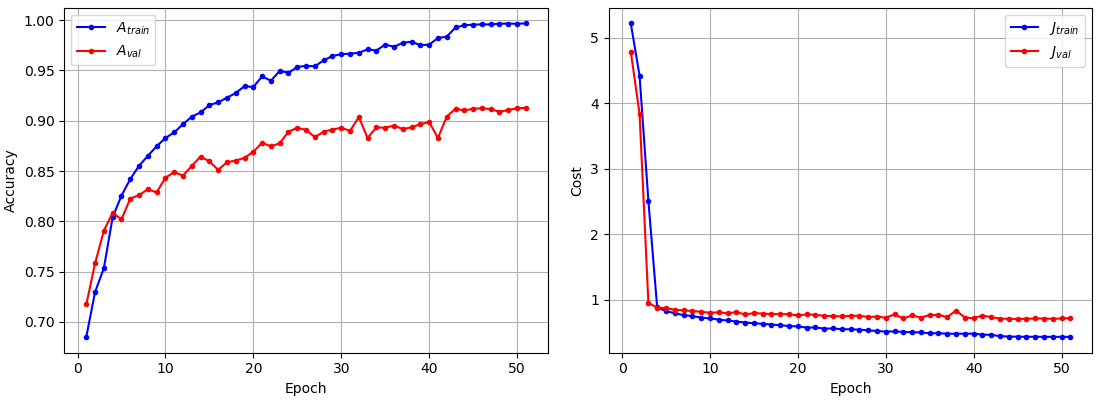
\includegraphics[width=0.8\textwidth]{figs/vgg16_partial_convergence.png}
    \caption{Partial feature extraction network (with $e = 14$, $f = 14$, $\lambda = 0.00015445$, $\eta = 10^{-4}$) converging to very good performance and modest model size.}
    \label{fig:vgg16_partial_convergence}
\end{figure}

% TODO: proof adam optimizer

A more thorough systematic study of the learning rate when extracting lower-level layers would certainly unveil more models with a good balance between model size and model performance, perhaps even outperforming models that extract all convolutional layers.

\subsection{Total Feature Extraction with Fine Tuning}

Presumably, further fine-tuning layers while extracting all $e = 18$ layers will yield higher performance since it will continue to optimize parameters relative to the target dataset thus minimizing error on said dataset.

Indeed, freezing the first $f = 14$ layers (versus the previous $e = f = 18$ configuration) yields a 2\% increase in accuracy on the test set (table \ref{table:vgg16_finetuning_14}).

\begin{table}[ht]
\centering
\begin{tabular}{ |c|c|c|c|c|c|c|c|c|c| }
\hline
$e$ & $f$ & $\lambda$ & $A_{train}$ & $A_{val}$ & $A_{test}$ & Precision & Recall & F1-Score \\
\hline
18 & 14 & 0.0001 & 1.0 & 0.928 & 0.934 & 0.936 & 0.934 & 0.934 \\
18 & 14 & 0.000154 & 1.0 & 0.923 & 0.94 & 0.941 & 0.94 & 0.94 \\
18 & 14 & 0.000239 & 1.0 & 0.925 & 0.939 & 0.94 & 0.939 & 0.939 \\
18 & 14 & 0.000368 & 1.0 & 0.926 & 0.939 & 0.94 & 0.939 & 0.939 \\
18 & 14 & 0.000569 & 1.0 & 0.925 & 0.941 & 0.942 & 0.941 & 0.941 \\
18 & 14 & 0.000879 & 1.0 & 0.921 & 0.929 & 0.93 & 0.929 & 0.929 \\
18 & 14 & 0.00136 & 1.0 & 0.923 & 0.938 & 0.94 & 0.938 & 0.938 \\
18 & 14 & 0.0021 & 1.0 & 0.927 & 0.936 & 0.937 & 0.936 & 0.936 \\
18 & 14 & 0.00324 & 1.0 & 0.925 & 0.936 & 0.937 & 0.936 & 0.936 \\
18 & 14 & 0.005 & 1.0 & 0.925 & 0.936 & 0.937 & 0.936 & 0.936 \\
\hline
 & & & $1.0\pm0.0$ & $0.925\pm0.00194$ & $0.937\pm0.00331$ & $0.938\pm0.00329$ & $0.937\pm0.00331$ & $0.937\pm0.00331$ \\
\hline
\end{tabular}
\caption{Performance metrics of models when $e = 18$ and $f = 14$.}
\label{table:vgg16_finetuning_14}
\end{table}

However, as $f$ decreases (to take values $f = 10$, $f = 6$, $f = 3$, and $f = 0$) the trend seems to be that performance declines (tables \ref{table:vgg16_finetuning_10}, \ref{table:vgg16_finetuning_6}, \ref{table:vgg16_finetuning_3}, and \ref{table:vgg16_finetuning_0} respectively).

\begin{table}[ht]
\centering
\begin{tabular}{ |c|c|c|c|c|c|c|c|c|c| }
\hline
$e$ & $f$ & $\lambda$ & $A_{train}$ & $A_{val}$ & $A_{test}$ & Precision & Recall & F1-Score \\
\hline
18 & 10 & 0.0001 & 0.5 & 0.5 & 0.5 & 0.25 & 0.5 & 0.334 \\
18 & 10 & 0.000154 & 1.0 & 0.926 & 0.934 & 0.935 & 0.934 & 0.934 \\
18 & 10 & 0.000239 & 1.0 & 0.928 & 0.931 & 0.933 & 0.931 & 0.931 \\
18 & 10 & 0.000368 & 1.0 & 0.922 & 0.931 & 0.932 & 0.931 & 0.931 \\
18 & 10 & 0.000569 & 1.0 & 0.933 & 0.943 & 0.945 & 0.943 & 0.943 \\
18 & 10 & 0.000879 & 1.0 & 0.925 & 0.93 & 0.931 & 0.93 & 0.93 \\
18 & 10 & 0.00136 & 1.0 & 0.935 & 0.937 & 0.938 & 0.937 & 0.937 \\
18 & 10 & 0.0021 & 1.0 & 0.931 & 0.927 & 0.928 & 0.927 & 0.927 \\
18 & 10 & 0.00324 & 1.0 & 0.929 & 0.94 & 0.941 & 0.94 & 0.94 \\
18 & 10 & 0.005 & 1.0 & 0.929 & 0.932 & 0.933 & 0.932 & 0.932 \\
\hline
 & & & $0.95\pm0.15$ & $0.886\pm0.129$ & $0.891\pm0.13$ & $0.867\pm0.206$ & $0.891\pm0.13$ & $0.874\pm0.18$ \\
\hline
\end{tabular}
\caption{Performance metrics of models when $e = 18$ and $f = 10$.}
\label{table:vgg16_finetuning_10}
\end{table}

\begin{table}[ht]
\centering
\begin{tabular}{ |c|c|c|c|c|c|c|c|c|c| }
\hline
$e$ & $f$ & $\lambda$ & $A_{train}$ & $A_{val}$ & $A_{test}$ & Precision & Recall & F1-Score \\
\hline
18 & 6 & 0.0001 & 0.5 & 0.5 & 0.5 & 0.25 & 0.5 & 0.333 \\
18 & 6 & 0.000154 & 0.5 & 0.5 & 0.5 & 0.25 & 0.5 & 0.333 \\
18 & 6 & 0.000239 & 1.0 & 0.93 & 0.927 & 0.928 & 0.927 & 0.927 \\
18 & 6 & 0.000368 & 0.5 & 0.5 & 0.5 & 0.25 & 0.5 & 0.333 \\
18 & 6 & 0.000569 & 1.0 & 0.925 & 0.927 & 0.928 & 0.927 & 0.927 \\
18 & 6 & 0.000879 & 1.0 & 0.922 & 0.928 & 0.929 & 0.928 & 0.928 \\
18 & 6 & 0.00136 & 0.5 & 0.501 & 0.499 & 0.416 & 0.499 & 0.334 \\
18 & 6 & 0.0021 & 0.501 & 0.498 & 0.5 & 0.5 & 0.5 & 0.336 \\
18 & 6 & 0.00324 & 1.0 & 0.917 & 0.916 & 0.917 & 0.916 & 0.916 \\
18 & 6 & 0.005 & 1.0 & 0.922 & 0.926 & 0.927 & 0.926 & 0.926 \\
\hline
 & & & $0.75\pm0.25$ & $0.711\pm0.212$ & $0.712\pm0.213$ & $0.629\pm0.306$ & $0.712\pm0.213$ & $0.629\pm0.296$ \\
\hline
\end{tabular}
\caption{Performance metrics of models when $e = 18$ and $f = 6$.}
\label{table:vgg16_finetuning_6}
\end{table}

\begin{table}[ht]
\centering
\begin{tabular}{ |c|c|c|c|c|c|c|c|c|c| }
\hline
$e$ & $f$ & $\lambda$ & $A_{train}$ & $A_{val}$ & $A_{test}$ & Precision & Recall & F1-Score \\
\hline
18 & 3 & 0.0001 & 1.0 & 0.9 & 0.913 & 0.913 & 0.913 & 0.913 \\
18 & 3 & 0.000154 & 0.5 & 0.5 & 0.5 & 0.25 & 0.5 & 0.333 \\
18 & 3 & 0.000239 & 0.5 & 0.5 & 0.5 & 0.25 & 0.5 & 0.333 \\
18 & 3 & 0.000368 & 1.0 & 0.915 & 0.924 & 0.925 & 0.924 & 0.924 \\
18 & 3 & 0.000569 & 1.0 & 0.926 & 0.931 & 0.932 & 0.931 & 0.931 \\
18 & 3 & 0.000879 & 1.0 & 0.927 & 0.933 & 0.934 & 0.933 & 0.933 \\
18 & 3 & 0.00136 & 1.0 & 0.933 & 0.931 & 0.933 & 0.931 & 0.931 \\
18 & 3 & 0.0021 & 1.0 & 0.931 & 0.932 & 0.933 & 0.932 & 0.932 \\
18 & 3 & 0.00324 & 0.5 & 0.5 & 0.5 & 0.25 & 0.5 & 0.334 \\
18 & 3 & 0.005 & 0.5 & 0.5 & 0.5 & 0.25 & 0.5 & 0.333 \\
\hline
 & & & $0.8\pm0.245$ & $0.753\pm0.207$ & $0.756\pm0.209$ & $0.657\pm0.332$ & $0.756\pm0.209$ & $0.69\pm0.291$ \\
\hline
\end{tabular}
\caption{Performance metrics of models when $e = 18$ and $f = 3$.}
\label{table:vgg16_finetuning_3}
\end{table}

\begin{table}[ht]
\centering
\begin{tabular}{ |c|c|c|c|c|c|c|c|c|c| }
\hline
$e$ & $f$ & $\lambda$ & $A_{train}$ & $A_{val}$ & $A_{test}$ & Precision & Recall & F1-Score \\
\hline
18 & 0 & 0.0001 & 0.5 & 0.5 & 0.5 & 0.25 & 0.5 & 0.333 \\
18 & 0 & 0.000154 & 1.0 & 0.916 & 0.923 & 0.923 & 0.923 & 0.923 \\
18 & 0 & 0.000239 & 1.0 & 0.9 & 0.906 & 0.907 & 0.906 & 0.906 \\
18 & 0 & 0.000368 & 0.5 & 0.5 & 0.5 & 0.25 & 0.5 & 0.333 \\
18 & 0 & 0.000569 & 0.5 & 0.5 & 0.5 & 0.25 & 0.5 & 0.333 \\
18 & 0 & 0.000879 & 0.501 & 0.5 & 0.499 & 0.25 & 0.499 & 0.333 \\
18 & 0 & 0.00136 & 0.5 & 0.5 & 0.5 & 0.25 & 0.5 & 0.333 \\
18 & 0 & 0.0021 & 0.5 & 0.5 & 0.5 & 0.25 & 0.5 & 0.333 \\
18 & 0 & 0.00324 & 0.5 & 0.5 & 0.5 & 0.25 & 0.5 & 0.333 \\
18 & 0 & 0.005 & 0.5 & 0.5 & 0.5 & 0.25 & 0.5 & 0.333 \\
\hline
 & & & $0.6\pm0.2$ & $0.582\pm0.163$ & $0.583\pm0.166$ & $0.383\pm0.266$ & $0.583\pm0.166$ & $0.449\pm0.233$ \\
\hline
\end{tabular}
\caption{Performance metrics of models when $e = 18$ and $f = 0$.}
\label{table:vgg16_finetuning_0}
\end{table}

This can be explained by an inadequate setting of the learning rate just as in the previous set of experiments. The more higher layers are unfrozen, the more their weights are disrupted too quickly because of too high a learning rate.

% TODO: proof different learning rate
% TODO: proof different optimizer

\section{End-to-End Learning Experiments}

This section describes a set of experiments involving models of custom designed \ac{CNN} architectures trained from scratch, following the more traditional methodology typically called end-to-end learning, that will be used for comparison against the transfer learning approach which it is in direct contrast with.

Designing a custom \ac{CNN} architecture from scratch is quite difficult as it requires setting and reasoning about many different hyperparameters simultaneously (number of convolutional layers, number of filters in each layer, size of filters, stride, etc.) for which there is no one right answer; hyperparameters should always be cross-validated from a wide range on the problem at hand. Instead, these custom architectures will be based around reasonable heuristics \cite{cs231n} extrapolated from the training of successful deep networks:

\begin{itemize}
    \item The most common architecture of convolutional neural networks is to stack ReLU-activated convolutional layers followed by a max pooling layer, a pattern which is arbitrarily repeated to some desired depth in order to reduce the dimensions of the features, after which it is common to use fully-connected layers;
    \item Prefer a stack of many small filters in convolutional layers rather than one large filter;
    \item Use zero-padding and stride $S = 1$ in convolutional layers as they provide better performance;
    \item Prefer $2 \times 2$ filters with stride $S = 2$ in pooling layers to avoid aggressive, lossy downsampling and consequently worse performance.
\end{itemize}

\subsection{Custom Architecture 1}

This custom architecture, illustrated in figure \ref{fig:custom1}, stacks three convolution-pooling blocks. Each block stacks two convolutional layers before the pooling layer, which is a good idea for large and deep networks because multiple stacked convolutional layers can develop more complex features of the input volume before the destructive pooling operation. Specifically,

\begin{enumerate}
    \item 32 $3 \times 3$ filters, stride of 1, zero padding, ReLU activated
    \item 32 $3 \times 3$ filters, stride of 1, zero padding, ReLU activated
    \item $2 \times 2$ max pooling with stride 2
    \item 64 $3 \times 3$ filters, stride of 1, zero padding, ReLU activated
    \item 64 $3 \times 3$ filters, stride of 1, zero padding, ReLU activated
    \item $2 \times 2$ max pooling with stride 2
    \item 128 $3 \times 3$ filters, stride of 1, zero padding, ReLU activated
    \item 128 $3 \times 3$ filters, stride of 1, zero padding, ReLU activated
\end{enumerate}

The classifier, illustrated in figure \ref{fig:custom1}, is a stack of two fully-connected layers of ReLU-activated neurons followed by a fully-connected sigmoid-activated neuron for binary classification.

\begin{enumerate}
    \item $u$ fully-connected ReLU-activated neurons;
    \item Another $u$ fully-connected ReLU-activated neurons;
    \item Single fully-connected sigmoid-activated neuron for binary classification.
\end{enumerate}

\begin{figure}[ht]
    \centering
    \includegraphics[width=1.0\textwidth]{figs/custom1.png}
    \caption{Architecture of the first custom-designed neural network.}
    \label{fig:custom1}
\end{figure}

Models of this architecture are trained identically as follows:

\begin{enumerate}
    \item Standardize training and validation samples relative to \ac{ISIC} 2018;
    \item Parameters are all initialized according to Xavier initialization;
    \item Define network architecture:
        \begin{enumerate}
            \item Stack blocks of convolutional and pooling layers to build useful features for classification;
            \item Use global average pooling to reduce the number of parameters before the classifier based on fully-connected layers;
            \item Stack fully-connected layers of ReLU-activated neurons;
            \item Add fully-connected layer with a single sigmoid-activated neuron for binary classification.
        \end{enumerate}
    \item Mini-batch \ac{SGD} with momentum $\gamma = 0.9$:
        \begin{itemize}
            \item Binary cross entropy cost function and explicit L2 regularization;
            \item 32 samples batches;
            \item Shuffle the $m$ samples every epoch;
            \item Initial learning rate $\eta = 10^{-4}$ that decays by a factor of $10$ if the validation accuracy has not improved $+10^{-3}$ in the last $10$ epochs;
            \item Train for a maximum of 1000 epochs, stopping early if the loss has not changed $\pm 10^{-3}$ in the last $30$ epochs.
        \end{itemize}
    \item Grid-search model selection based on the accuracy as measured on a fixed validation set;
    \item Final models will be evaluated and compared primarily using accuracy as measured on the test set.
\end{enumerate}

The L2-regularization strength $\lambda$ is cross-validated from $\lambda \in [0.0001, 0.005]$ spaced evenly on a log scale. Results are summarized in table \ref{table:custom1_all}.

\begin{table}[ht]
\centering
\begin{tabular}{ |c|c|c|c|c|c|c|c| }
\hline
$\lambda$ & $A_{train}$ & $A_{val}$ & $A_{test}$ & Precision & Recall & F1-Score \\
\hline
0.0001 & 0.737 & 0.726 & 0.741 & 0.756 & 0.741 & 0.737 \\
0.000154 & 0.734 & 0.724 & 0.737 & 0.755 & 0.737 & 0.732 \\
0.000239 & 0.795 & 0.785 & 0.781 & 0.785 & 0.781 & 0.78 \\
0.000368 & 0.782 & 0.768 & 0.772 & 0.78 & 0.772 & 0.771 \\
0.000569 & 0.723 & 0.72 & 0.729 & 0.753 & 0.729 & 0.722 \\
0.000879 & 0.724 & 0.72 & 0.729 & 0.755 & 0.729 & 0.722 \\
0.00136 & 0.723 & 0.718 & 0.729 & 0.753 & 0.729 & 0.722 \\
0.0021 & 0.721 & 0.716 & 0.728 & 0.753 & 0.728 & 0.721 \\
0.00324 & 0.719 & 0.709 & 0.724 & 0.75 & 0.724 & 0.717 \\
0.005 & 0.713 & 0.704 & 0.718 & 0.745 & 0.718 & 0.71 \\
\hline
 & $0.737\pm0.0267$ & $0.729\pm0.0248$ & $0.739\pm0.0199$ & $0.758\pm0.0124$ & $0.739\pm0.0199$ & $0.733\pm0.0223$ \\
\hline
\end{tabular}
\caption{Performance metrics of models of the custom architecture 1 where $\lambda$ is varied.}
\label{table:custom1_all}
\end{table}

The effect of $\lambda$ on the performance of the model can be understood in figure \ref{fig:custom1_lambda}.

\begin{figure}[ht]
    \centering
    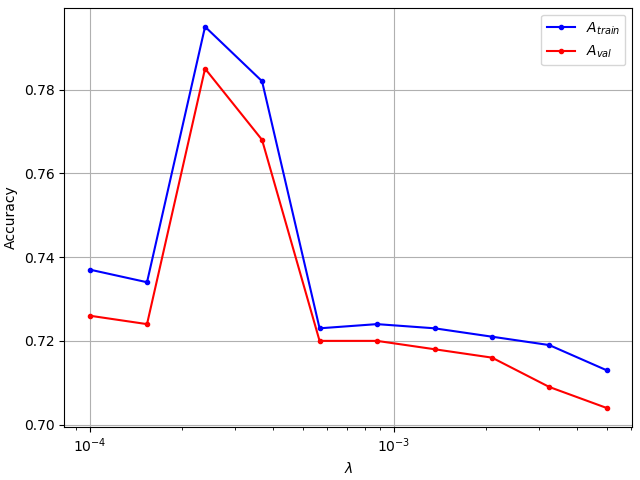
\includegraphics[width=0.8\textwidth]{figs/custom1_lambda.png}
    \caption{Accuracy on the test set $A_{test}$ of models of the custom architecture 1 over a range of values for L2-regularization strength $\lambda$.}
    \label{fig:custom1_lambda}
\end{figure}

In particular, $\lambda = 0.000239$ gives the best performing model of the custom architecture 1. The convergence of this model can be tracked in figure \ref{fig:custom1_best_training} and the final confusion matrix in figure \ref{fig:custom1_best_confusionmatrix}.

\begin{figure}[ht]
    \centering
    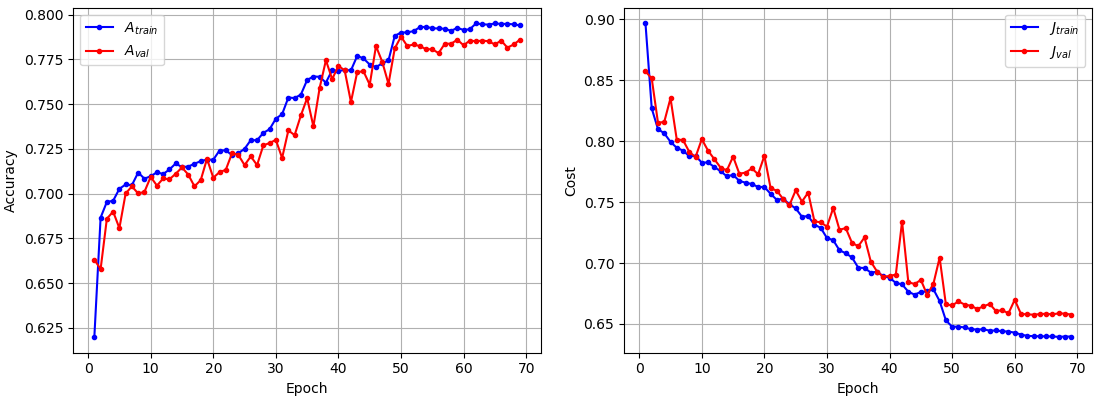
\includegraphics[width=0.8\textwidth]{figs/custom1_best_training.png}
    \caption{Convergence of the best model of the custom architecture 1.}
    \label{fig:custom1_best_training}
\end{figure}

\begin{figure}[ht]
    \centering
    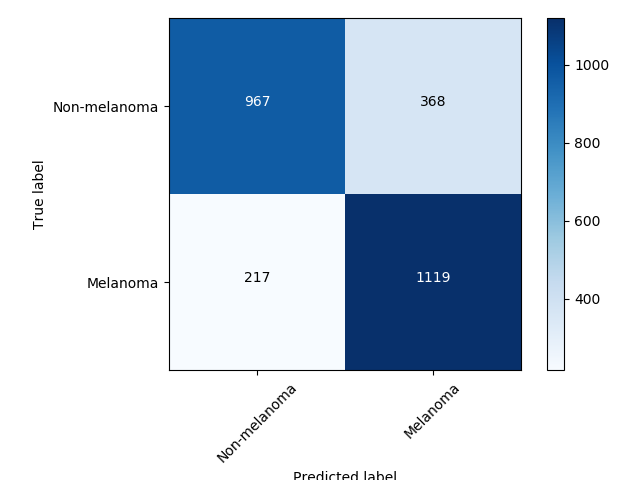
\includegraphics[width=0.8\textwidth]{figs/custom1_best_confusionmatrix.png}
    \caption{Confusion matrix of the best model of the custom architecture 1.}
    \label{fig:custom1_best_confusionmatrix}
\end{figure}

\subsection{Custom Architecture 2}

This custom architecture, illustrated in figure \ref{fig:custom2}, stacks two convolution-pooling blocks. Each block uses a single convolutional layer before the pooling layer:

\begin{enumerate}
    \item 32 $3 \times 3$ filters, stride of 1, zero padding, ReLU activated;
    \item $2 \times 2$ max pooling with stride of 2;
    \item 64 $3 \times 3$ filters, stride of 1, zero padding, ReLU activated;
    \item $2 \times 2$ max pooling with stride of 2.
\end{enumerate}

The classifier is a single fully-connected layer of $u$ ReLU-activated neurons followed by a fully-connected sigmoid-activated neuron for binary classification:

\begin{enumerate}
    \item $u$ fully-connected ReLU-activated neurons;
    \item Single fully-connected sigmoid-activated neuron for binary classification.
\end{enumerate}

\begin{figure}[ht]
    \centering
    \includegraphics[width=1.0\textwidth]{figs/custom2.png}
    \caption{Custom Architecture 2.}
    \label{fig:custom2}
\end{figure}

Models of this architecture are trained identically as follows:

\begin{enumerate}
    \item Standardize training and validation samples relative to \ac{ISIC} 2018;
    \item Parameters are all initialized according to Xavier initialization;
    \item Define network architecture:
        \begin{enumerate}
            \item Stack blocks of convolutional and pooling layers to build useful features for classification;
            \item Use global average pooling to reduce the number of parameters before the classifier based on fully-connected layers;
            \item Stack fully-connected layers of ReLU-activated neurons;
            \item Add fully-connected layer with a single sigmoid-activated neuron for binary classification.
        \end{enumerate}
    \item Mini-batch \ac{SGD} with momentum $\gamma = 0.9$:
        \begin{itemize}
            \item Binary cross entropy cost function and explicit L2 regularization;
            \item 32 samples batches;
            \item Shuffle the $m$ samples every epoch;
            \item Initial learning rate $\eta = 10^{-4}$ that decays by a factor of $10$ if the validation accuracy has not improved $+10^{-3}$ in the last $10$ epochs;
            \item Train for a maximum of 1000 epochs, stopping early if the loss has not changed $\pm 10^{-3}$ in the last $30$ epochs.
        \end{itemize}
    \item Grid-search model selection based on the accuracy as measured on a fixed validation set;
    \item Final models will be evaluated and compared primarily using accuracy as measured on the test set.
\end{enumerate}

The L2-regularization strength $\lambda$ is cross-validated from $\lambda \in [0.0001, 0.005]$ spaced evenly on a log scale. Results are summarized in table \ref{table:custom2_all}.

\begin{table}[ht]
\centering
\begin{tabular}{ |c|c|c|c|c|c|c|c| }
\hline
$\lambda$ & $A_{train}$ & $A_{val}$ & $A_{test}$ & Precision & Recall & F1-Score \\
\hline
0.0001 & 0.737 & 0.724 & 0.736 & 0.756 & 0.736 & 0.73 \\
0.000154 & 0.736 & 0.72 & 0.735 & 0.757 & 0.735 & 0.729 \\
0.000239 & 0.734 & 0.72 & 0.737 & 0.76 & 0.737 & 0.731 \\
0.000368 & 0.731 & 0.717 & 0.738 & 0.761 & 0.738 & 0.732 \\
0.000569 & 0.724 & 0.716 & 0.735 & 0.762 & 0.735 & 0.728 \\
0.000879 & 0.724 & 0.719 & 0.736 & 0.764 & 0.736 & 0.729 \\
0.00136 & 0.725 & 0.719 & 0.735 & 0.754 & 0.735 & 0.729 \\
0.0021 & 0.718 & 0.71 & 0.729 & 0.756 & 0.729 & 0.722 \\
0.00324 & 0.714 & 0.706 & 0.721 & 0.752 & 0.721 & 0.712 \\
0.005 & 0.711 & 0.703 & 0.717 & 0.753 & 0.717 & 0.707 \\
\hline
 & $0.725\pm0.00865$ & $0.715\pm0.00645$ & $0.732\pm0.00689$ & $0.758\pm0.00385$ & $0.732\pm0.00689$ & $0.725\pm0.00818$ \\
\hline
\end{tabular}
\caption{Performance metrics of models of the custom architecture 2 where $\lambda$ is varied.}
\label{table:custom2_all}
\end{table}

The effect of $\lambda$ on the performance of the model can be understood in figure \ref{fig:custom2_lambda}.

\begin{figure}[ht]
    \centering
    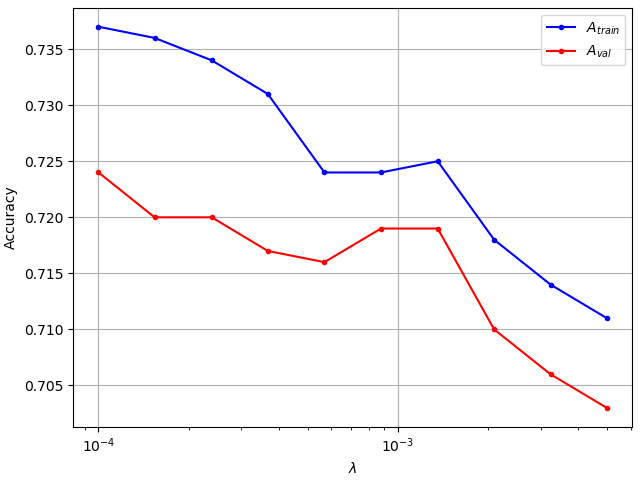
\includegraphics[width=0.8\textwidth]{figs/custom2_lambda.png}
    \caption{Accuracy on the test set $A_{test}$ of models of the custom architecture 2 over a range of values for L2-regularization strength $\lambda$.}
    \label{fig:custom2_lambda}
\end{figure}

In particular, $\lambda = 0.0003684$ gives the best performing model of the custom architecture 2. The convergence of this model can be tracked in figure \ref{fig:custom2_best_training} and the final confusion matrix in figure \ref{fig:custom2_best_confusionmatrix}.

\begin{figure}[ht]
    \centering
    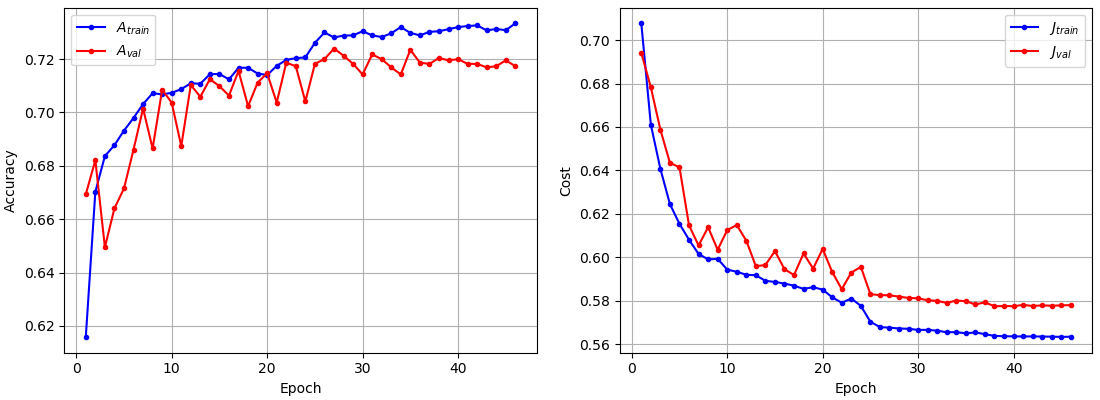
\includegraphics[width=0.8\textwidth]{figs/custom2_best_training.png}
    \caption{Convergence of the best model of the custom architecture 2.}
    \label{fig:custom2_best_training}
\end{figure}

\begin{figure}[ht]
    \centering
    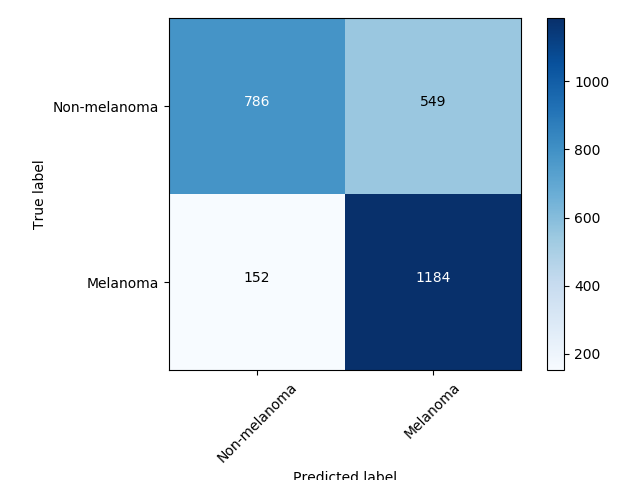
\includegraphics[width=0.8\textwidth]{figs/custom2_best_confusionmatrix.png}
    \caption{Confusion matrix of the best model of the custom architecture 2.}
    \label{fig:custom2_best_confusionmatrix}
\end{figure}

\section{Discussion}

% TODO: why is custom1 better than custom2?

% TODO: plot sobreposto de A_test de melhores modelos de cada tipo

